\documentclass[12pt]{book}
%\documentclass[journal,5pt,twocolumn]{IEEEtran}
%\makeatletter
\usepackage{tikz}
\usetikzlibrary{shapes,arrows}
\makeatother
\usepackage{setspace}
\usepackage{gensymb}
\usepackage{xcolor}
\usepackage{caption}
%\usepackage{stackengine}
%\usepackage{subcaption}
%\doublespacing
\usepackage{xcolor}
\usepackage{lipsum}
\singlespacing
\def\baselinestretch{1.5}
\usepackage{fancyhdr}
\pagestyle{fancy}
\fancyhf{} 

%\counterwithin{enumi}{section}
%\counterwithin{equation}{enumi}
%\counterwithin{figure}{enumi}

\newcommand\figref{Fig.~\ref}
\usepackage[colorlinks=true, allcolors=black]{hyperref}

\usepackage{graphicx}
%\graphicspath{ {./images}  }
%\usepackage{amssymb}
%\usepackage{relsize}
\usepackage[cmex10]{amsmath}
\usepackage{mathtools}
%\usepackage{amsthm}
\interdisplaylinepenalty=2500
%\savesymbol{iint}
%\usepackage{txfonts}
%\restoresymbol{TXF}{iint}
\usepackage{wasysym}
\usepackage{amsthm}
\usepackage{mathrsfs}
\usepackage{txfonts}
\usepackage{stfloats}
\usepackage{cite}
\usepackage{cases}
\usepackage{mathtools}
\usepackage{subfig}
\usepackage{enumerate}	
\usepackage{enumitem}
\usepackage{amsmath}
%\usepackage{xtab}
\usepackage{longtable}
\usepackage{multirow}
%\usepackage{algorithm}
%\usepackage{algpseudocode}
\usepackage{enumitem}
\usepackage{mathtools}
\usepackage{tikz}
\usetikzlibrary{shapes,arrows,automata,petri,positioning,calc}
%\usetikzlibrary{arrows.meta,calc,positioning}
%\usepackage[framemethod=tikz]{mdframed}
\usepackage{listings}
    \usepackage[latin1]{inputenc}                                 %%
    \usepackage{color}                                            %%
    \usepackage{array}                                            %%
    \usepackage{longtable}                                        %%
    \usepackage{calc}                                             %%
    \usepackage{multirow}                                         %%
    \usepackage{hhline}                                           %%
    \usepackage{ifthen}                                           %%
  %optionally (for landscape tables embedded in another document): %%
    \usepackage{lscape}     


%\usepackage{stmaryrd}


%\usepackage{wasysym}
%\newcounter{MYtempeqncnt}
\DeclareMathOperator*{\Res}{Res}
%\renewcommand{\baselinestretch}{4}
%\setcounter{secnumdepth}{4}
\renewcommand\thesection{\arabic{section}}
\renewcommand\thesubsection{\thesection.\arabic{subsection}}
\renewcommand\thesubsubsection{\thesubsection.\arabic{subsubsection}}
%\renewcommand\thesubsubsubsection{\thesubsubsection.\arabic{subsubsubsection}}


\hyphenation{Future Wireless communications}

%\lstset{
%language=C,
%frame=single, 
%breaklines=true
%}

\def\inputGnumericTable{}                                 %%

\lstset{
%language=python,
frame=single, 
breaklines=true,
columns=fullflexible
}

 \usepackage{watermark}

\begin{document}
%
\tikzstyle{block} = [rectangle, draw,
text width=7em, text centered, minimum height=4em]
\tikzstyle{sum} = [draw, circle, node distance=3cm]
\tikzstyle{input} = [coordinate]
\tikzstyle{output} = [coordinate]
\tikzstyle{pinstyle} = [pin edge={to-,thin,black}]
\tikzstyle{line} = [draw, -latex']
\theoremstyle{definition}
\newtheorem{theorem}{Theorem}[section]
\newtheorem{problem}{Problem}
\newtheorem{proposition}{Proposition}[section]
\newtheorem{lemma}{Lemma}[section]
\newtheorem{corollary}[theorem]{Corollary}
\newtheorem{example}{Example}[section]
\newtheorem{definition}{Definition}[section]
%\newtheorem{algorithm}{Algorithm}[section]
%\newtheorem{cor}{Corollary}
\newcommand{\BEQA}{\begin{eqnarray}}
\newcommand{\EEQA}{\end{eqnarray}}
\newcommand{\define}{\stackrel{\triangle}{=}}
\bibliographystyle{IEEEtran}
%\bibliographystyle{ieeetr}
\providecommand{\nCr}[2]{\,^{#1}C_{#2}} % nCr
\providecommand{\nPr}[2]{\,^{#1}P_{#2}} % nPr
\providecommand{\mbf}{\mathbf}
\providecommand{\pr}[1]{\ensuremath{\Pr\left(#1\right)}}
\providecommand{\qfunc}[1]{\ensuremath{Q\left(#1\right)}}
\providecommand{\sbrak}[1]{\ensuremath{{}\left[#1\right]}}
\providecommand{\lsbrak}[1]{\ensuremath{{}\left[#1\right.}}
\providecommand{\rsbrak}[1]{\ensuremath{{}\left.#1\right]}}
\providecommand{\brak}[1]{\ensuremath{\left(#1\right)}}
\providecommand{\lbrak}[1]{\ensuremath{\left(#1\right.}}
\providecommand{\rbrak}[1]{\ensuremath{\left.#1\right)}}
\providecommand{\cbrak}[1]{\ensuremath{\left\{#1\right\}}}
\providecommand{\lcbrak}[1]{\ensuremath{\left\{#1\right.}}
\providecommand{\rcbrak}[1]{\ensuremath{\left.#1\right\}}}
\theoremstyle{remark}
\newtheorem{rem}{Remark}
\newcommand{\sgn}{\mathop{\mathrm{sgn}}}
\providecommand{\abs}[1]{\left\vert#1\right\vert}
\providecommand{\res}[1]{\Res\displaylimits_{#1}} 
\providecommand{\norm}[1]{\lVert#1\rVert}
\providecommand{\mtx}[1]{\mathbf{#1}}
\providecommand{\mean}[1]{E\left[ #1 \right]}
\providecommand{\fourier}{\overset{\mathcal{F}}{ \rightleftharpoons}}
%\providecommand{\hilbert}{\overset{\mathcal{H}}{ \rightleftharpoons}}
\providecommand{\system}{\overset{\mathcal{H}}{ \longleftrightarrow}}
	%\newcommand{\solution}[2]{\textbf{Solution:}{#1}}
\newcommand{\solution}{\noindent \textbf{Solution: }}
\newcommand{\myvec}[1]{\ensuremath{\begin{pmatrix}#1\end{pmatrix}}}
\providecommand{\dec}[2]{\ensuremath{\overset{#1}{\underset{#2}{\gtrless}}}}
\DeclarePairedDelimiter{\ceil}{\lceil}{\rceil}
%\numberwithin{equation}{subsection}
\numberwithin{equation}{section}
%\numberwithin{problem}{subsection}
%\numberwithin{definition}{subsection}
%\makeatletter
%\@addtoreset{figure}{section}
%\makeatother
\let\StandardTheFigure\thefigure
%\renewcommand{\thefigure}{\theproblem.\arabic{figure}}
%\renewcommand{\thefigure}{\thesection}
%\numberwithin{figure}{subsection}
%\numberwithin{equation}{subsection}
%\numberwithin{equation}{section}
%\numberwithin{equation}{problem}
%\numberwithin{problem}{subsection}
%\numberwithin{problem}{section}
%%\numberwithin{definition}{subsection}
%\makeatletter
%\@addtoreset{figure}{problem}
%\makeatother
%\makeatletter
%\@addtoreset{table}{problem}
%\makeatother
\let\StandardTheFigure\thefigure
\let\StandardTheTable\thetable
\let\vec\mathbf
%%\renewcommand{\thefigure}{\theproblem.\arabic{figure}}
%\renewcommand{\thefigure}{\theproblem}
%%\numberwithin{figure}{section}
%%\numberwithin{figure}{subsection}
\def\putbox#1#2#3{\makebox[0in][l]{\makebox[#1][l]{}\raisebox{\baselineskip}[0in][0in]{\raisebox{#2}[0in][0in]{#3}}}}
     \def\rightbox#1{\makebox[0in][r]{#1}}
     \def\centbox#1{\makebox[0in]{#1}}
     \def\topbox#1{\raisebox{-\baselineskip}[0in][0in]{#1}}
     \def\midbox#1{\raisebox{-0.5\baselineskip}[0in][0in]{#1}}
\title{ 
%	\logo{
FREQUENCY MODULATION
%	}
}
\author{ Under guidance of Dr. GVV SHARMA}% <-this % stops a space
\thiswatermark{\centering \put(-50,-105){
\includegraphics[scale=0.5]{iith.png}}}
% make the title area
\maketitle
\tableofcontents

\chapter{FREQUENCY MODULATION}
\section{Message}

The message signal is available in 
\begin{lstlisting}
fm/msg/codes/Sound_Noise.wav
\end{lstlisting}
\begin{enumerate}[label=\arabic*.,ref=\thesection.\theenumi]
\numberwithin{equation}{enumi}
\item Plot the spectrum of the message signal.\\
Solution:
The spectrum of input audio signal is plotted in \figref{fig:input_spectrum} using below code

\begin{center}
\fcolorbox{red}{white}{\parbox{7.5cm}
{\href{https://github.com/Gangagopinath/fwc/tree/main/FM/code}
{/codes/input.py}}}
\end{center}

%\begin{enumerate}
%\item 
To plot the spectrum of the message signal, we need to compute the Fourier Transform of the message signal, which will give us the frequency domain representation of the signal.

\begin{equation}
M_k = \sum_{n=0}^{N-1} m(n) e^{-j2\pi kn/N}, \quad k=0,1,\dots,N-1
\end{equation}
In code for computing the FFT of m(n)
\begin{equation}
M_k = \texttt{fft}(x(n), N)
\end{equation}
\iffalse
\begin{align*}
M(f) = FFT(m(n))
\end{align*}
\fi
%\end{enumerate}
Where $M_k$ is the frequency representation of the signal, m(n) is the input signal. 
\item Find the bandwidth of the message signal.\\
\solution:
\begin {enumerate}
\item By calculating the Power Spectral Density: 
\begin{align*}
PSD(M)=\lvert M(k) \rvert^2 
\end{align*}
Where PSD(M) is the power spectral density at frequency f, M(K) is the Fourier Transform of the input signal

\item Finding the Frequency Range with Significant Power:

\begin{align*}
mask(f) &=
\begin{cases}
 1 \quad PSD(f) > T\\
0 \quad otherwise
\end{cases}
\end{align*}


\begin{figure}
\centering 
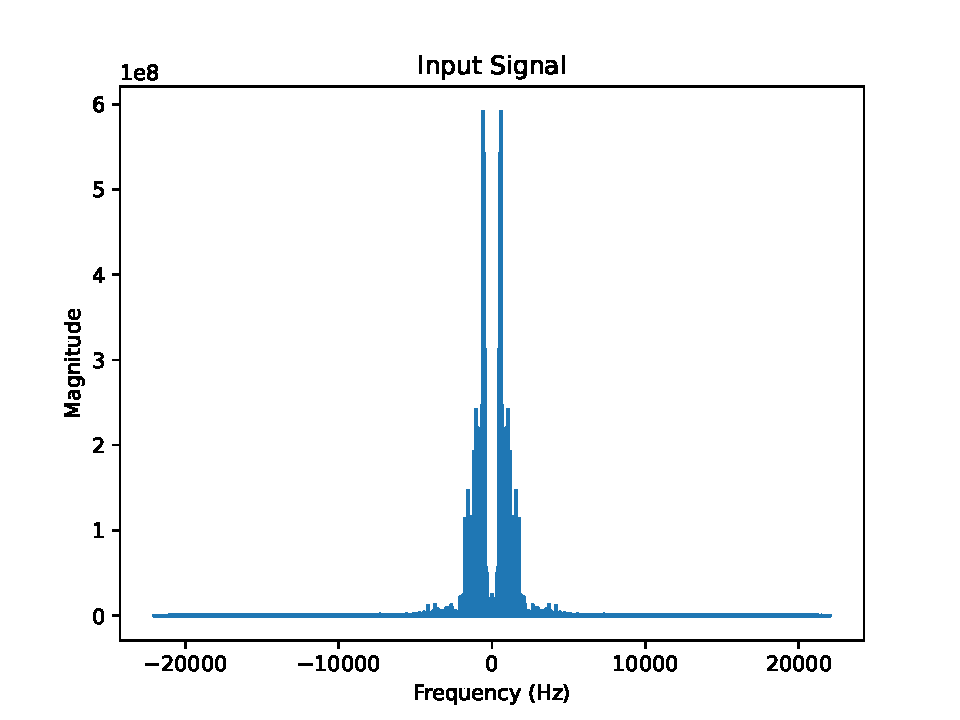
\includegraphics[width=\columnwidth]{./inputs.pdf}
\caption{spectrum analysis of input signal}
\label{fig:input_spectrum}
\end{figure}

\end{enumerate}
 Bandwidth  is calculate as the difference between the maximum and minimum frequencies in the range with significant power.
\begin{align*}
B = f_u - f_l
\end{align*}
where $f_l $ and $f_u $arethe lower and upper frequency bounds of the range  respectively.
\
\end{enumerate}

\section{Transmitter}
\begin{enumerate}
\item The modulated signal is given by 
\begin{align}
	s(t) = \cos\brak{2\pi f_c t + \phi(t)}
\end{align}
where
\begin{align}
	\phi(t) = 2\pi k_f \int_{0}^{t}m(\tau)\,d\tau
	\label{phi}
\end{align}
List the various parameters in a table.\\
\vspace{10mm}
\begin{tabular}{|c|l|c|}
    \hline 
    \textbf{Parameter} & \textbf{Value} &\textbf{Description} \\ \hline
    T&0.1&Threshold\\
    $K_{f}$ & 20 Hz/volt & Frequency sensitivity \\ 
    $A_c$ & 1  & amplitude of the carrier signal\\ 
    $F_c $& 100 MHz & Frequency of the carrier signal\\ 
    $F_s$ & 44100 Hz & Sampling rate\\ 
    t     & 22 $\mu$ & Sampling time\\  \hline
    \end{tabular}
\\


\item Obtain a difference equation for computing $\phi(t)$.  Suggest a sampling rate.\\

\solution \quad To obtain the difference equation for computing $\phi(t)$, we need to discretize the integral in the given equation. We can use the rectangular rule for numerical integration.\\ 

Let us divide the interval $[t_0, t]$ into $N$ equal subintervals of width $\Delta t = (t - t_0)/N$. Then, we can approximate $m(\tau)$ by its value at the midpoint of each subinterval, $\tau_n = t_0 + (n + 1/2)\Delta t$, where $n = 0, 1, 2, ..., N-1$. This gives:
\begin{align*}
m(\tau_n) \approx m(n\Delta t)
\end{align*}
we can approximate the integral in the given equation \ref{phi}
\begin{align*}
\phi(t) \approx 2\pi kf_c \Delta t \sum_{n=0}^{N-1} m(n\Delta t)
\end{align*}
$\phi$ at the $n$th time step $t_n = t_0 + n\Delta t$. Then, we can write:
\begin{equation}
\label{n}
\phi_n = 2\pi kf_c \Delta t \sum_{k=0}^{n-1} m(k\Delta t) \\
\end{equation}
\begin{equation}
\label{n-1}
\phi_{n-1} = 2\pi kf_c \Delta t \sum_{k=0}^{n-2} m(k\Delta t)
\end{equation}
Subtracting the \ref{n-1} from \ref{n}, we get:
\begin{equation}
\phi_n - \phi_{n-1} = 2\pi k_f f_c \Delta t, m((n-1)\Delta t)
\end{equation}
\item Plot the spectrum of the transmitted signal.\\
Solution:\quad The spectrum of FM signal is plotted in \figref{fig:fm_spectrum} using below code


\begin{center}
\fcolorbox{red}{white}{\parbox{7.5cm}
{\href{https://github.com/Gangagopinath/fwc/tree/main/FM/code}
{/codes/mod.py}}}
\end{center}

 \begin{figure}
\centering 
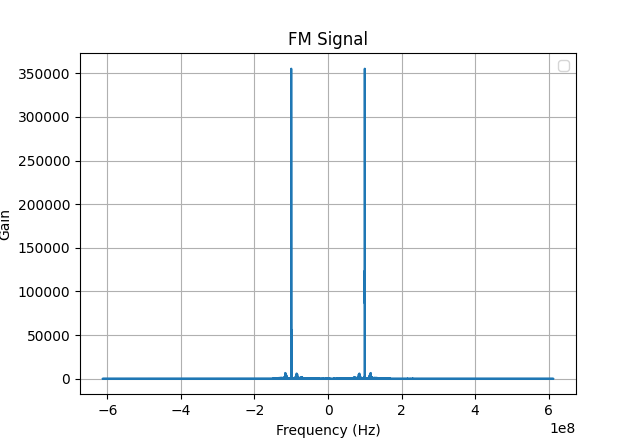
\includegraphics[width=\columnwidth]{./fm.png}
\caption{spectrum analysis of fm signal}
\label{fig:fm_spectrum}
\end{figure}

\item Compute the bandwidth of the transmitted signal.\\
Solution:\\By computing the Fourier Transform:
\begin{equation}
S_k = \sum_{n=0}^{N-1} s(n) e^{-j2\pi kn/N}, \quad k=0,1,\dots,N-1
\end{equation}
In code for computing the FFT of s(n)
\begin{equation}
S_k = \texttt{fft}(s(n), N)
\end{equation}
Where $S_k$ is the frequency representation of the signal, s(n) is the transmitted signal. 
\item Find the bandwidth of the message signal.\\
solution: \quad we need to calculate its power spectral density. This can be done using the equation \eqref{eq:psd}

Calculating the Power Spectral Density: 
\begin{align}
PSD(s)=\lvert S_k \rvert^2 
\label{eq:psd}
\end{align}
we can identify the frequency range with significant power using a mask function. 
\begin{align*}
mask(s) &=
\begin{cases}
 1 \quad PSD(s) > T\\
0 \quad otherwise
\end{cases}
\end{align*}
Bandwidth can then be calculated as
\begin{align*}
B = f_u - f_l
\end{align*}
where $f_l $ and $f_u $arethe lower and upper frequency bounds of the range  respectively.

\end{enumerate}
\end{document}